\section{Calibration and validation}\label{sec:calib}

Table~\ref{tab:params} in Appendix~\ref{app:params} lists every parameter with its value and source. Issuer sizes
and reserve mixes are defaults from public attestations (\$180\,bn for Issuer~A with 66\% bills, 10\% reverse
repo, 4\% money market funds, 0.5\% cash and 19.5\% other assets; \$75\,bn for Issuer~B with 12\% deposits and
the rest in a government fund holding 40\% bills and 48\% repo on a look-through basis); both are flagged for
verification. Market-side parameters (impact coefficients, dealer capacity, reinvestment) are anchored on the
literature or set by assumption and varied in Section~\ref{sec:robust}.

The behavioural and plumbing parameters that the literature does not pin down are calibrated on two episodes. The
USDC episode of March 2023 is represented, for Issuer~B, as an 8\% exposure with no processing on business day~1
(the weekend) and resolution on day~2; targets are a trough of 0.87--0.88, redemptions of 12--15\% of supply in
the first week and about 25\% after a month. The USDT episode of May 2022 is represented, for Issuer~A, as a
feared exposure resolved after ten days of successful redemptions; targets are a trough of 0.95--0.97 and
redemptions of about 12\% in two weeks. All targets are from memory and listed for verification. A two-stage grid
fits the shared parameters (liquidity depth $\eta$, a common scale on the exit thresholds, the depeg weight $w_1$,
the loss probability $\psi$ and the size of the feared USDT exposure) jointly with issuer-specific processing
capacity and arbitrage capital, minimising the sum of squared standardised target errors. The best fit has
$\eta=0.1$, threshold scale~1, $w_1=0.5$, $\psi=1$, a feared USDT exposure of 2\%, processing capacity of 1.2\% of
supply per day for Issuer~A and 3\% for Issuer~B, and arbitrage capital of 1.1\% and 3\% of supply per day.

\begin{table}[tbp]\centering\small
\caption{Validation against the two calibration episodes (300 paths, 10{,}000 agents). $z$ is the model minus the
observed value in units of the tolerance. All observed values are to be verified.}\label{tab:validation}
\resizebox{\textwidth}{!}{\begin{tabular}{llrrr}
\toprule
Episode & Target & Observed (tol.) & Model & $z$ \\
\midrule
USDC, March 2023 (Issuer B) & Minimum price & 0.875 (0.010) & 0.904 & +2.9 \\
USDC, March 2023 (Issuer B) & Redeemed, 5 business days & 0.135 (0.015) & 0.120 & -1.0 \\
USDC, March 2023 (Issuer B) & Redeemed, 22 business days & 0.250 (0.030) & 0.240 & -0.3 \\
USDT, May 2022 (Issuer A) & Minimum price & 0.960 (0.015) & 0.925 & -2.3 \\
USDT, May 2022 (Issuer A) & Redeemed, 10 business days & 0.120 (0.015) & 0.120 & -0.0 \\
\bottomrule
\end{tabular}
}
\end{table}

\begin{figure}[tbp]\centering
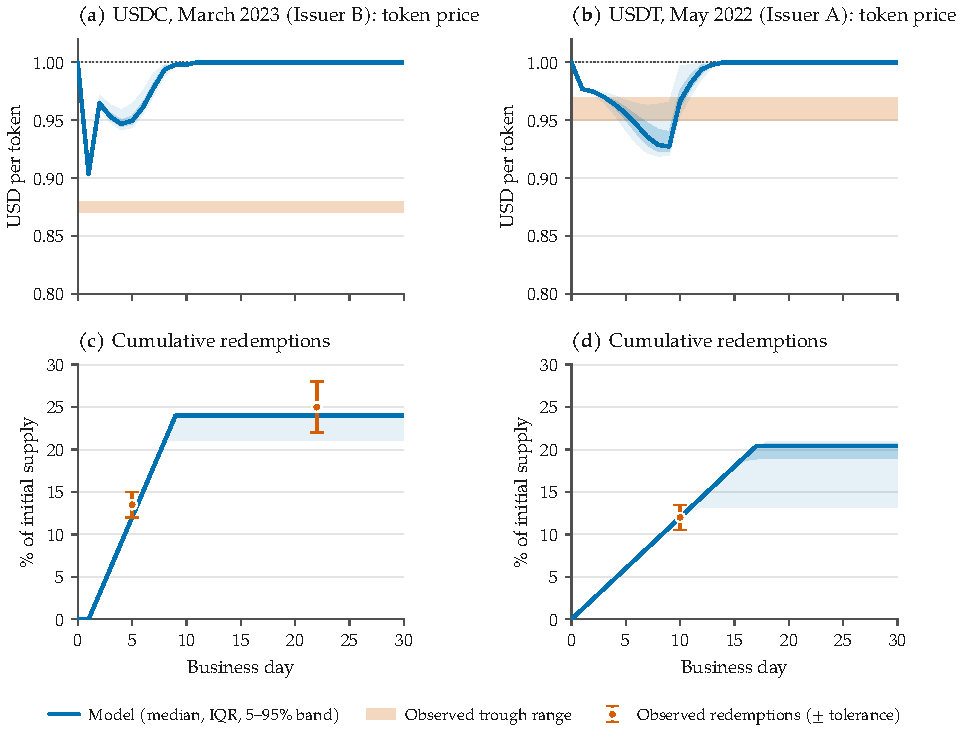
\includegraphics[width=\textwidth]{F4_validation}
\caption{Validation. Model paths (median, interquartile range and 5--95\% band) for the token price and cumulative
redemptions in the two calibration episodes, against the observed trough range and redemption targets (to be
verified).}\label{fig:f4}
\end{figure}

Table~\ref{tab:validation} and Figure~\ref{fig:f4} show the fit. Redemption volumes are matched in both episodes:
12\% of USDC supply in the first week against 12--15\% observed, 24\% after a month against 25\%, and 12\% of USDT
supply in two weeks. Processing capacity is the binding constraint in both, which is why the fitted capacities
are low: 1.2\% of supply per day is about \$2\,bn for Issuer~A, close to what Tether actually paid out per day in
May 2022, and 3\% is about \$2.3\,bn for Issuer~B. The model under-predicts the depth of the USDC trough (0.90
against 0.875) and over-predicts that of USDT (0.93 against 0.96); a single liquidity-depth parameter cannot
reproduce both a thin weekend crypto market with banks closed and a deep weekday market. We report this as a
limitation rather than add a weekend-specific parameter, and note that the discrepancy affects the price channel
only: the bill-market results below depend on redemption volumes and timing, which are matched.

\section{Results}\label{sec:results}

\subsection{Baseline dynamics (E1)}

\begin{figure}[tbp]\centering
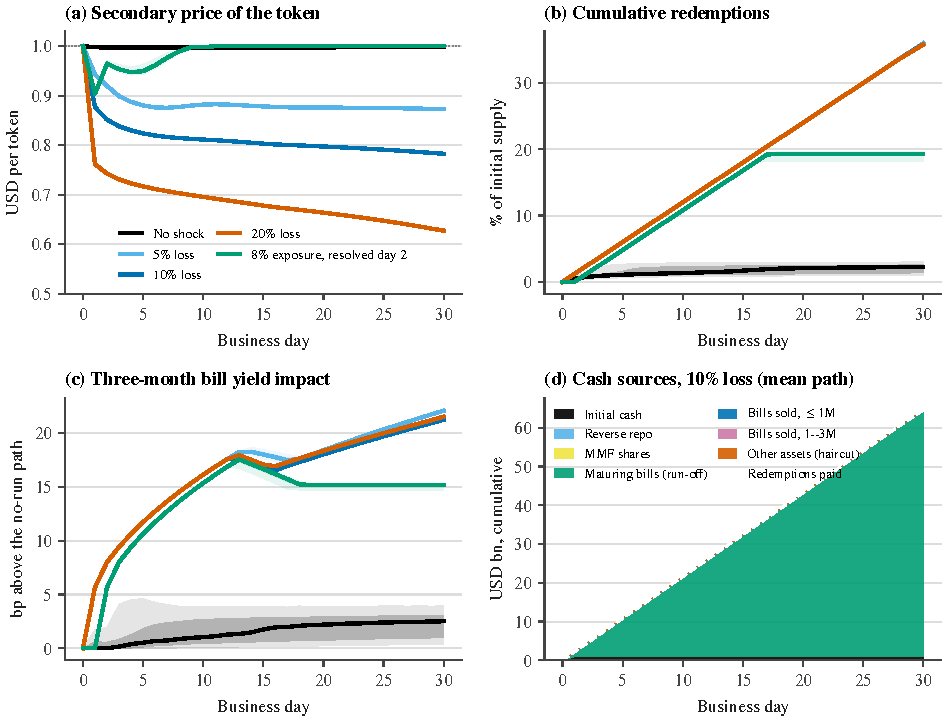
\includegraphics[width=\textwidth]{F1_A_baseline_dynamics}
\caption{Baseline run dynamics for Issuer~A (1{,}000 paths; lines are medians, bands the interquartile and 5--95\%
ranges). (a)~Secondary price; (b)~cumulative redemptions; (c)~three-month bill-yield impact; (d)~cash sources that
funded redemptions in the 10\% loss scenario (mean path): the dashed line is cumulative redemptions paid.}
\label{fig:f1}
\end{figure}

\begin{table}[tbp]\centering\small
\caption{E1 baseline, Issuer~A, 1{,}000 Monte Carlo paths, 30 business days. Medians across paths unless stated.
``Resolved'' = 8\% of reserves exposed, no processing on day~1, exposure resolved without loss on day~2.}
\label{tab:e1}
\resizebox{\textwidth}{!}{\begin{tabular}{@{}lrrrrr@{}}
\toprule
 & No shock & 5\% loss & 10\% loss & 20\% loss & \begin{tabular}[b]{@{}r@{}}8\% exposure,\\resolved day 2\end{tabular} \\
\midrule
\multicolumn{6}{@{}l}{\itshape Run} \\
\quad Minimum token price & 0.997 & 0.872 & 0.783 & 0.628 & 0.904 \\
\quad Redeemed by day 7 & 1.2\% & 8.4\% & 8.4\% & 8.4\% & 7.2\% \\
\quad Redeemed by day 30 & 2.2\% & 36.0\% & 35.8\% & 35.8\% & 19.3\% \\
\quad P(redemptions $\geq$ 20\%) & 0\% & 100\% & 100\% & 100\% & 0\% \\
\quad P(redemptions $\geq$ 50\%) & 0\% & 0\% & 0\% & 0\% & 0\% \\
\quad P(any suspension day) & 0\% & 0\% & 0\% & 0\% & 0\% \\
\addlinespace
\multicolumn{6}{@{}l}{\itshape Treasury-bill market} \\
\quad Peak three-month yield impact, bp & 4.2 & 22.1 & 21.2 & 21.5 & 17.5 \\
\quad Peak impact, bp, 95th percentile & 5.8 & 22.2 & 21.3 & 21.5 & 17.6 \\
\quad Bills sold outright, \$bn & 0.0 & 0.0 & 0.0 & 0.0 & 0.0 \\
\quad Maturing bills not rolled, \$bn & 3.1 & 66.1 & 63.5 & 64.3 & 33.9 \\
\quad Peak net bill demand withdrawn, \$bn & 2.1 & 34.8 & 32.2 & 33.1 & 22.0 \\
\addlinespace
\multicolumn{6}{@{}l}{\itshape Issuer} \\
\quad Other assets sold, \$bn & 0.0 & 0.0 & 0.0 & 0.0 & 0.0 \\
\quad Fire-sale and haircut loss, \$bn & 0.00 & 0.00 & 0.00 & 0.00 & 0.00 \\
\quad Net asset value on day 30 & 1.000 & 0.923 & 0.845 & 0.690 & 1.000 \\
\bottomrule
\end{tabular}
}
\end{table}

Figure~\ref{fig:f1} and Table~\ref{tab:e1} show Issuer~A under five shocks: no shock, a realised loss of 5, 10 or
20\% of reserves, and the calibrated liquidity scare. Three features stand out. First, a realised loss of any size
in this range produces a run: redemptions reach 8.4\% of supply in the first week and 36\% by day 30 in all three
loss scenarios, and the probability of a run is one. The run is not larger because it cannot be faster:
processing capacity binds for the first three weeks and arbitrage capital thereafter, so the loss scenarios
differ only in price, which settles at one minus the loss share of the remaining holders minus a liquidity
discount (0.87, 0.78 and 0.63 for the 5, 10 and 20\% losses) and keeps drifting down as the loss concentrates on
those who stay. Second, the liquidity scare looks different: the price falls to 0.90 while redemption is closed,
recovers fully within two weeks as re-entering holders absorb the overhang, and redemptions stop at 19\% of
supply, just below the run threshold. Third, and most important for the Treasury market, the issuer sells no bills
outright in any scenario. Panel~(d) shows why: with processing capacity of about \$2.2\,bn a day and \$2.8\,bn of bills
maturing every business day, every dollar of redemptions is paid out of run-off, and reverse repo and money market
fund shares are never touched. The issuer stops rolling those maturities while it has pending claims; over the month it withholds \$63\,bn of auction demand in the 10\% loss scenario, about half of
which returns through money market funds, for a peak net demand withdrawal of \$32\,bn and a peak three-month
yield impact of 21\,bp. The fire-sale loss is zero because nothing is sold, and even where bills are sold in
later experiments it stays below \$10\,m: a bill with six weeks to maturity sold 60\,bp cheap loses seven basis
points of face value. The externality falls on the Treasury market, not on the issuer.

Issuer~B behaves differently (Appendix~\ref{app:extra}, Table~\ref{tab:e1B}). Its reserves contain no cushion of
other assets to absorb an impairment, so a realised loss hits deposits and the fund directly; with faster
processing (3\% a day) it pays out 80--90\% of supply within the month in the loss scenarios, sells up to \$8\,bn
of bills once repo is exhausted, and suspends in the 10\% and 20\% loss scenarios when the remaining holders are
left with nothing. Its liquidity scare ends with 24\% of supply redeemed, the USDC outcome it was calibrated to.

\subsection{Tipping point (E2)}

\begin{figure}[tbp]\centering
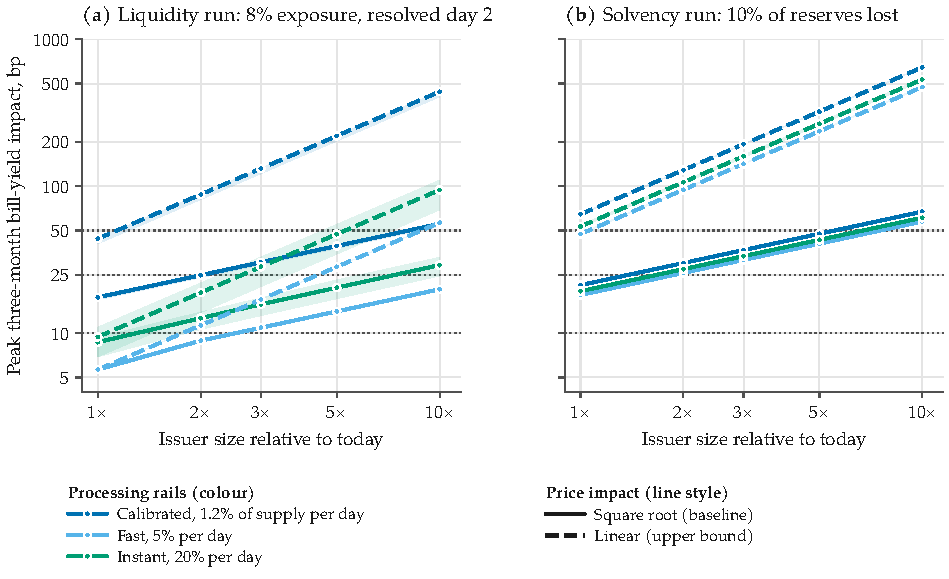
\includegraphics[width=\textwidth]{F2_tipping_point}
\caption{Peak three-month bill-yield impact against issuer size (log scales, medians with 5--95\% bands, 300
paths). ``Rails'' is daily processing capacity as a share of supply: calibrated (1.2\%), fast (5\%) or instant
(20\%). Dotted lines mark 10, 25 and 50\,bp.}\label{fig:f2}
\end{figure}

\begin{table}[tbp]\centering\small
\caption{E2: median peak three-month bill-yield impact (bp) by issuer size, and the size at which it first exceeds
10, 25 and 50\,bp (log-linear interpolation). Issuer~A, 300 paths per cell.}\label{tab:e2}
\resizebox{\textwidth}{!}{\begin{tabular}{@{}lllrrrrrrrr@{}}
\toprule
 &  &  & \multicolumn{5}{c}{\begin{tabular}[b]{@{}c@{}}Peak impact, bp,\\at issuer size\end{tabular}} & \multicolumn{3}{c@{}}{\begin{tabular}[b]{@{}c@{}}Size at which\\impact first exceeds\end{tabular}} \\
\cmidrule(lr){4-8}\cmidrule(l){9-11}
Scenario & Price impact & Rails & 1$\times$ & 2$\times$ & 3$\times$ & 5$\times$ & 10$\times$ & 10 bp & 25 bp & 50 bp \\
\midrule
Liquidity run & Square root & Calibrated & 18 & 25 & 30 & 39 & 55 & $<1\times$ & 2.0$\times$ & 8.1$\times$ \\
 &  & Fast & 6 & 9 & 11 & 14 & 20 & 2.5$\times$ & $>10\times$ & $>10\times$ \\
 &  & Instant & 9 & 13 & 16 & 20 & 29 & 1.3$\times$ & 7.4$\times$ & $>10\times$ \\
 & Linear & Calibrated & 44 & 88 & 132 & 220 & 440 & $<1\times$ & $<1\times$ & 1.1$\times$ \\
 &  & Fast & 6 & 11 & 17 & 28 & 57 & 1.8$\times$ & 4.4$\times$ & 8.8$\times$ \\
 &  & Instant & 9 & 19 & 28 & 47 & 94 & 1.1$\times$ & 2.6$\times$ & 5.3$\times$ \\
\addlinespace
Solvency run & Square root & Calibrated & 21 & 30 & 37 & 47 & 67 & $<1\times$ & 1.4$\times$ & 5.5$\times$ \\
 &  & Fast & 18 & 26 & 32 & 41 & 58 & $<1\times$ & 1.9$\times$ & 7.5$\times$ \\
 &  & Instant & 19 & 27 & 33 & 43 & 61 & $<1\times$ & 1.7$\times$ & 6.7$\times$ \\
 & Linear & Calibrated & 64 & 129 & 193 & 322 & 644 & $<1\times$ & $<1\times$ & $<1\times$ \\
 &  & Fast & 47 & 95 & 142 & 237 & 473 & $<1\times$ & $<1\times$ & 1.1$\times$ \\
 &  & Instant & 53 & 107 & 160 & 266 & 533 & $<1\times$ & $<1\times$ & $<1\times$ \\
\bottomrule
\end{tabular}
}
\end{table}

Figure~\ref{fig:f2} and Table~\ref{tab:e2} scale Issuer~A to 2, 3, 5 and 10 times its current size, holding the
bill market fixed and scaling everything on the issuer's side (processing capacity, arbitrage capital, the ladder)
with it, so that the exercise isolates the market's capacity to absorb. Under square-root impact the peak yield
effect grows with roughly the square root of size: a solvency run moves three-month yields by 21\,bp today, 30\,bp
at twice today's size, 47\,bp at five times and 67\,bp at ten times; the liquidity scare moves them by 18, 25, 39
and 55\,bp. The 25\,bp threshold is crossed at 1.4 times today's size for a solvency run and 2 times for a scare;
the 50\,bp threshold at 5.5 and 8 times. Under linear impact, the upper bound in which every billion withdrawn costs
the same two basis points, both thresholds are crossed already at today's size and a tenfold issuer would move the
front end by several hundred basis points, a dislocation that would certainly trigger intervention.

Redemption speed matters, but not in the direction one might expect. Faster rails (5\% or 20\% of supply per day)
produce \emph{more} redemptions (52\% of supply instead of 36\% in a solvency run) but a \emph{smaller} yield
impact at small sizes: when the issuer can pay quickly it pays from cash and repo, the redeemed cash reaches money
market funds within two days and comes back to the bill market, and the net demand withdrawn is small. Slow rails
keep the issuer in a weeks-long state of pending claims in which it hoards maturities, so the slow configuration
withholds \$34\,bn of auction demand in a scare against \$18\,bn with fast rails. Only with instant rails and at
five to ten times today's size does the issuer sell bills outright in volume (\$24--48\,bn in a scare, \$27\,bn in a
solvency run), and even then dealer inventory never approaches its capacity because money-market-fund reinvestment
buys what dealers would otherwise warehouse. The dealer-capacity channel, which dominated March 2020, is
inactive in this model unless the reinvestment leak is closed (Section~\ref{sec:robust}).

\subsection{Policy levers (E3)}

\begin{table}[tbp]\centering\small
\caption{E3 policy grid: main effects. Each row averages the outcome over the other levers (96 cells per
configuration, 200 paths per cell). The liquidity run is at today's size with calibrated rails; the solvency run is
a 10\% loss at five times today's size with fast rails. ``Redemption basis'' rows are single runs without other
policies.}\label{tab:e3}
\resizebox{\textwidth}{!}{\begin{tabular}{@{}lrrrrrrrr@{}}
\toprule
 & \multicolumn{4}{c}{Liquidity run, today's size, calibrated rails} & \multicolumn{4}{c@{}}{Solvency run, 5$\times$ today's size, fast rails} \\
\cmidrule(lr){2-5}\cmidrule(l){6-9}
 & \begin{tabular}[b]{@{}r@{}}Impact,\\bp\end{tabular} & \begin{tabular}[b]{@{}r@{}}Redeemed\\by day 30\end{tabular} & \begin{tabular}[b]{@{}r@{}}Minimum\\price\end{tabular} & \begin{tabular}[b]{@{}r@{}}Bills sold,\\\$bn\end{tabular} & \begin{tabular}[b]{@{}r@{}}Impact,\\bp\end{tabular} & \begin{tabular}[b]{@{}r@{}}Redeemed\\by day 30\end{tabular} & \begin{tabular}[b]{@{}r@{}}Minimum\\price\end{tabular} & \begin{tabular}[b]{@{}r@{}}Bills sold,\\\$bn\end{tabular} \\
\midrule
\multicolumn{9}{@{}l}{\itshape Minimum cash buffer, share of reserves} \\
\quad 0\% & 7.1 & 19.4\% & 0.904 & 0 & 41.3 & 51.9\% & 0.747 & 153 \\
\quad 10\% & 4.3 & 19.4\% & 0.904 & 0 & 35.2 & 51.9\% & 0.747 & 65 \\
\quad 20\% & 0.0 & 19.4\% & 0.904 & 0 & 25.5 & 51.9\% & 0.747 & 14 \\
\quad 30\% & 0.0 & 19.4\% & 0.904 & 0 & 14.8 & 51.9\% & 0.747 & 0 \\
\addlinespace
\multicolumn{9}{@{}l}{\itshape Redemption fee} \\
\quad 0\% & 2.9 & 19.4\% & 0.904 & 0 & 30.3 & 51.9\% & 0.747 & 63 \\
\quad 0.5\% & 2.9 & 19.4\% & 0.904 & 0 & 29.7 & 51.9\% & 0.747 & 60 \\
\quad 1\% & 2.9 & 19.4\% & 0.904 & 0 & 29.0 & 51.9\% & 0.747 & 57 \\
\quad 2\% & 2.8 & 19.4\% & 0.904 & 0 & 27.9 & 51.9\% & 0.747 & 52 \\
\addlinespace
\multicolumn{9}{@{}l}{\itshape Maturity cap} \\
\quad 93 days & 5.2 & 19.4\% & 0.904 & 0 & 29.2 & 51.9\% & 0.747 & 3 \\
\quad 180 days & 3.1 & 19.4\% & 0.904 & 0 & 28.3 & 51.9\% & 0.747 & 47 \\
\quad None & 0.3 & 19.4\% & 0.904 & 0 & 30.1 & 51.9\% & 0.747 & 125 \\
\addlinespace
\multicolumn{9}{@{}l}{\itshape Fed backstop} \\
\quad Off & 3.8 & 19.4\% & 0.904 & 0 & 39.2 & 51.9\% & 0.747 & 58 \\
\quad On & 1.9 & 19.4\% & 0.904 & 0 & 19.3 & 51.9\% & 0.747 & 58 \\
\addlinespace
\multicolumn{9}{@{}l}{\itshape Redemption basis (single runs, no other policy)} \\
\quad Par & 17.6 & 19.4\% & 0.904 & 0 & 40.7 & 51.9\% & 0.747 & 13 \\
\quad Net asset value & 17.6 & 19.4\% & 0.904 & 0 & 36.9 & 52.6\% & 0.831 & 0 \\
\bottomrule
\end{tabular}
}
\end{table}

\begin{figure}[tbp]\centering
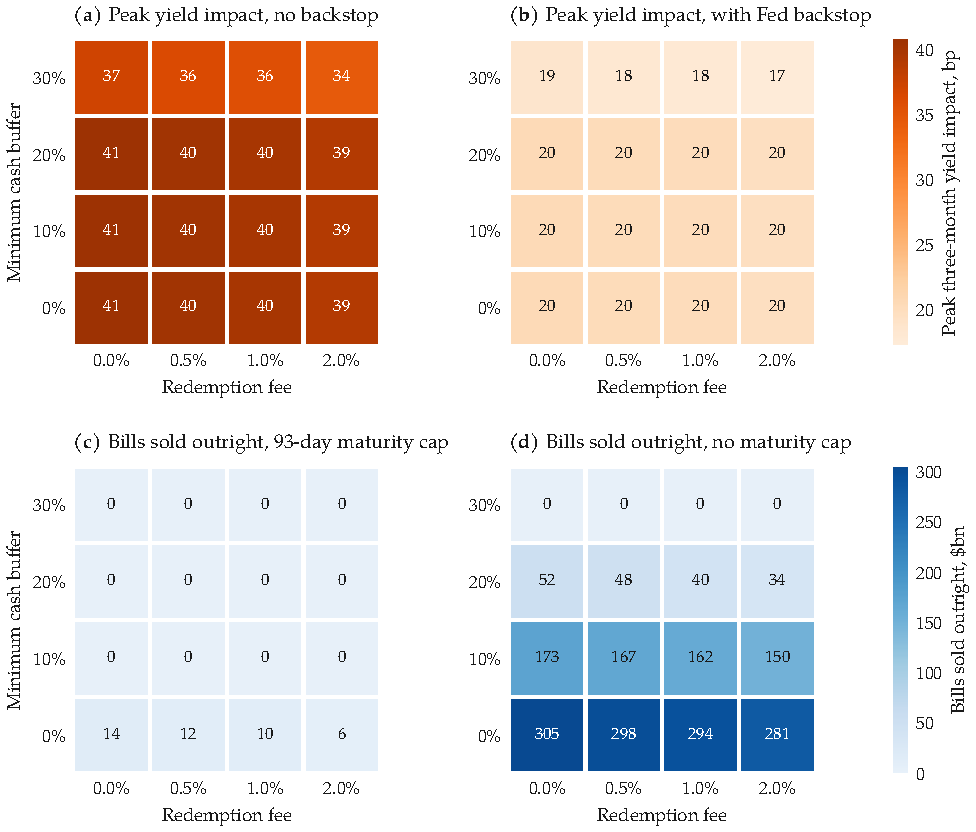
\includegraphics[width=0.92\textwidth]{F3_policy_heatmaps}
\caption{Policy grid for the solvency run at five times today's size with fast rails, by minimum cash buffer and
redemption fee. Top: peak bill-yield impact with the 93-day maturity cap, without and with a Fed backstop (shared
colour scale). Bottom: bills sold outright without a backstop, with the 93-day cap and with no cap.}\label{fig:f3}
\end{figure}

Table~\ref{tab:e3} and Figure~\ref{fig:f3} evaluate four levers on a full factorial grid, plus redemption at net
asset value, for a liquidity run at today's size and a solvency run at five times today's size with fast rails.
A \emph{minimum cash buffer} is the most powerful lever for the Treasury market: 20\% of reserves in cash removes
the bill-market footprint of the liquidity run entirely (from 7\,bp averaged over the grid to zero), and 30\% cuts
the solvency run's footprint from 41 to 15\,bp and the bills sold outright from \$153\,bn to zero, because the
buffer is spent before any bill is touched. It does nothing for the run itself: redemptions and the trough are
unchanged, since they are set by beliefs and processing. A \emph{maturity cap} trades one channel for the other:
with the 93-day cap the solvency run sells \$3\,bn of bills and withholds the rest through non-rollover, with a
180-day cap it sells \$47\,bn and with no cap \$125\,bn, while the measured yield impact barely changes because the
model prices withdrawn demand and outright sales alike. The cap therefore converts a dealer-balance-sheet event
into an auction-demand event, which is a gain in orderliness that the impact metric does not reward.
\emph{Redemption fees} of up to 2\% are ineffective: they shave two basis points off the impact and do not change
redemptions, because a holder facing a 10\% loss does not care about a 2\% fee and a scare resolves before the fee
binds. The \emph{Fed backstop} halves the footprint by construction (it halves the impact coefficients), so its
value in the model is the value of the assumption that a bill-purchase facility halves price impact; we include it
to show the scale of what a backstop must achieve rather than as a finding. Finally, \emph{redeeming at net asset
value} rather than par, the mutual-fund rule, does not stop the run (52.6\% against 51.9\% redeemed) but raises the
price trough from 0.75 to 0.83 and removes outright bill sales, because the loss no longer concentrates on those
who stay and the incentive to be first is weaker.

\subsection{Contagion (E4)}\label{sec:e4}

\begin{table}[tbp]\centering\small
\caption{E4 contagion: a shock to Issuer~A spills over to Issuer~B's beliefs with weight $\beta$ on A's depeg
(300 paths). ``Combined impact'' applies the persistent impact function to both issuers' net demand withdrawn.}
\label{tab:e4}
\resizebox{\textwidth}{!}{\begin{tabular}{@{}lrrrrrr@{}}
\toprule
 &  & \multicolumn{4}{c}{Issuer B} &  \\
\cmidrule(lr){3-6}
Shock to Issuer A & $\beta$ & \begin{tabular}[b]{@{}r@{}}Redeemed\\by day 7\end{tabular} & \begin{tabular}[b]{@{}r@{}}Redeemed\\by day 30\end{tabular} & \begin{tabular}[b]{@{}r@{}}Minimum\\price\end{tabular} & P(run) & \begin{tabular}[b]{@{}r@{}}Combined\\impact, bp\end{tabular} \\
\midrule
Liquidity run & 0.0 & 2.0\% & 2.3\% & 0.998 & 0\% & 17.5 \\
 & 0.3 & 14.0\% & 14.0\% & 0.967 & 9\% & 17.5 \\
 & 0.6 & 21.0\% & 30.0\% & 0.908 & 100\% & 17.5 \\
\addlinespace
Solvency run & 0.0 & 2.0\% & 2.3\% & 0.998 & 0\% & 21.2 \\
 & 0.3 & 21.0\% & 70.1\% & 0.879 & 100\% & 21.3 \\
 & 0.6 & 21.0\% & 90.0\% & 0.819 & 100\% & 21.2 \\
\bottomrule
\end{tabular}
}
\end{table}

Table~\ref{tab:e4} shocks Issuer~A and lets Issuer~B's holders add $\beta$ times A's depeg to their expected
loss. With $\beta=0.3$, a liquidity scare at A pulls 14\% of B's supply out at a trough of 0.97 and a solvency
run at A pulls 70\% out at 0.88; with $\beta=0.6$ B runs in every path. Yet the combined bill-market impact is
indistinguishable from A's alone, because B funds redemptions from deposits and repo and withdraws essentially no
bill demand. Contagion in this model is a peg and liquidity problem for the second issuer, not an additional
Treasury-market problem, as long as the second issuer's reserves are as liquid as Issuer~B's.

\section{Robustness}\label{sec:robust}

\begin{figure}[tbp]\centering
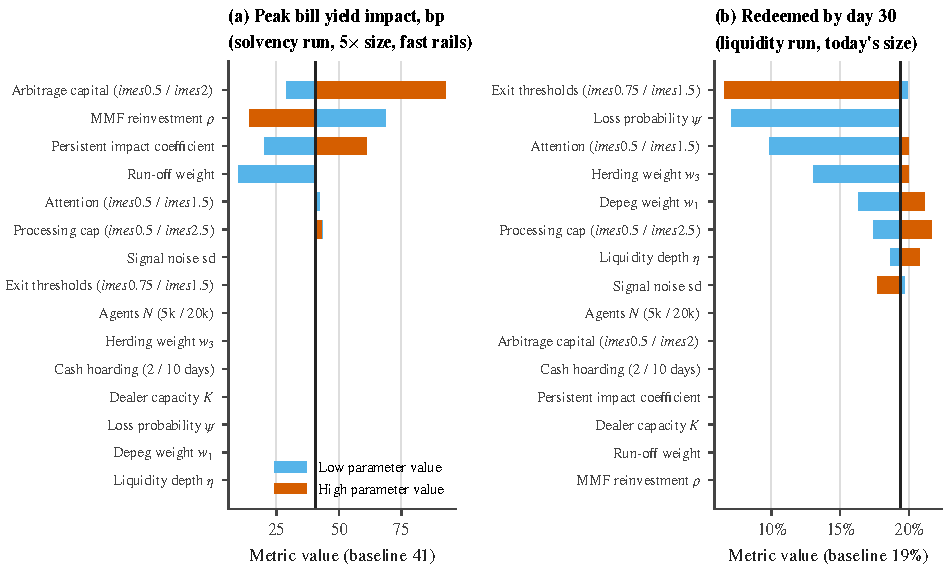
\includegraphics[width=\textwidth]{F5_sensitivity_tornado}
\caption{One-at-a-time sensitivity (200 paths). Bars show the change in the headline metric when each parameter is
moved to a low or high value, holding the others at baseline. (a)~Peak bill-yield impact in the solvency run at five
times today's size with fast rails; (b)~day-30 redemptions in the liquidity run at today's size.}\label{fig:f5}
\end{figure}

Figure~\ref{fig:f5} moves fifteen parameters one at a time between a low and a high value. The two panels tell
complementary stories. The Treasury-market footprint of a solvency run (panel~a) is governed by plumbing: the share
of redeemed cash that returns to bills through money market funds moves the peak impact between 14\,bp
($\rho=1$) and 69\,bp ($\rho=0$); the weight of non-rollover relative to a sale moves it between 10 and 41\,bp;
the persistent impact coefficient between 20 and 61\,bp; and arbitrage capital, which sets how fast the run can
proceed, between 29 and 93\,bp. The behavioural parameters (liquidity depth, thresholds, depeg and herding weights,
signal noise, attention) and dealer capacity move it by less than two basis points, and the number of agents by
none. The size of a liquidity run (panel~b) is the mirror image: day-30 redemptions range from 7\% to 20\% with
the threshold scale, from 10\% to 20\% with attention, from 7\% to 19\% with the loss probability $\psi$ and from
13\% to 20\% with herding, while every market-side parameter leaves them unchanged. The model's two halves are
separable, which is also why the imperfect fit of the price trough in Section~\ref{sec:calib} does not propagate
to the bill-market results.

Two further checks are in the appendices. Appendix~\ref{app:benchmark} shows that with the behavioural channels
off the simulation reproduces the closed-form threshold aggregate to within a tenth of a percentage point at every
loss share, so the heterogeneous-threshold machinery adds dynamics without distorting the static limit. The
linear-impact rows of Table~\ref{tab:e2} bound the results from above. Two robustness exercises in the
pre-registered design were not run: an hourly time step for the first five days, and a global (Sobol or Morris)
sensitivity design; the one-at-a-time design above is the first-order substitute and the hourly dynamics of the
USDC weekend are, as the validation showed, the part of the data the model fits least well.

\section{Policy implications}\label{sec:policy}

Five implications follow, each conditional on the model and on the verification of its inputs.

\emph{The channel is auction demand, not fire sales, at today's size.} An issuer with a self-liquidating bill ladder
and a processing throttle meets a run by not rolling maturities. The Treasury does not face a dealer dumping bills;
it faces a large buyer absent from the next several auctions. Monitoring should focus on issuers' rollover behaviour
and auction participation rather than on secondary-market sales, and the GENIUS Act's monthly reserve reports
should include ladder structure.

\emph{Size is the problem, and the threshold is not far.} Under the conservative square-root assumption, a run on an
issuer at one and a half to two times today's size moves three-month yields by 25\,bp, and at five to eight times by
50\,bp; under linear impact those marks are crossed today. The projections of a multi-trillion sector would, in this
model, put a stablecoin run in the same class as the March 2020 money market fund episode.

\emph{Cash buffers protect the Treasury market, not the peg.} A 20--30\% minimum cash share removes the footprint of
a liquidity run and most of a solvency run's, but changes nothing about how much is redeemed or how far the price
falls. Regulators who want to protect the bill market should mandate the buffer; those who want to protect holders
need the other levers.

\emph{Net-asset-value redemption weakens the stampede.} Paying at net asset value rather than par is the one lever
that improves the holder-side outcome, halving the depeg in a solvency run, because it removes the advantage of
being first. Redemption fees do not.

\emph{The reinvestment circuit is the key unknown.} Nothing in the model matters more for the Treasury market than
where redeemed cash goes. If it returns to bills through money market funds within days the system is a closed
circuit and the footprint is small; if it leaves for bank deposits or other assets the footprint quadruples and
dealer balance sheets come into play. This is an empirical question that the 2022 and 2023 episodes can answer and
that the model cannot.

\section{Conclusion}\label{sec:conclusion}

We built a calibrated agent-based stress test linking stablecoin run dynamics, redemption plumbing and Treasury-bill
price impact. At today's size a run on the largest issuer moves three-month bill yields by about 20\,bp through
withdrawn auction demand rather than fire sales, and the issuer's own fire-sale losses are negligible; the 25\,bp
mark is crossed at 1.4--2 times today's size and the 50\,bp mark at 5.5--8 times under square-root impact, and
already today under linear impact. Cash buffers and maturity caps shape the Treasury-market footprint, net-asset-value
redemption shapes the holder-side outcome, and fees shape neither. The model's two halves are separable: behaviour
sets the size of the run, plumbing sets its footprint.

The limitations are explicit. Reserve compositions and episode targets are from memory and must be verified;
the model fits redemption volumes well and price troughs less well; price impact is extrapolated from small
normal-times flows with a functional form that bounds rather than pins the answer; the dealer-capacity channel is
inactive unless reinvestment is slow; there are no inflows, no hourly dynamics and no bank-deposit channel; and the
model has two episodes of discipline. It is a stress-testing tool whose value lies in making the channels and the
orders of magnitude explicit, and in being reproducible: every number in this paper is regenerated from the
repository by one command.
